\section{Insight into Buck's Theorem}

\citet*{matousek:2002} gives two proofs for a simpler version of
\ref{theorem:xy:counting}. The second one is nice and visual, we
sketch it to give an insight into why \ref{theorem:xy:counting} holds
true.

The simpler theorem is the following
\begin{theorem}[Number of \(d\)-cells in an arrangement of hyperplanes]
Consider the partition of space defined by an arrangement of \(n\) hyperplanes
in \(\R^d\). The number of cells (or \(d\)-cells, regions of dimension \(d\))
is at most
\begin{displaymath}
\Phi_d(n) = \binom{n}{0} + \binom{n}{1} + \cdots + \binom{n}{d}
\end{displaymath}
\end{theorem}

\begin{figure}
\centering
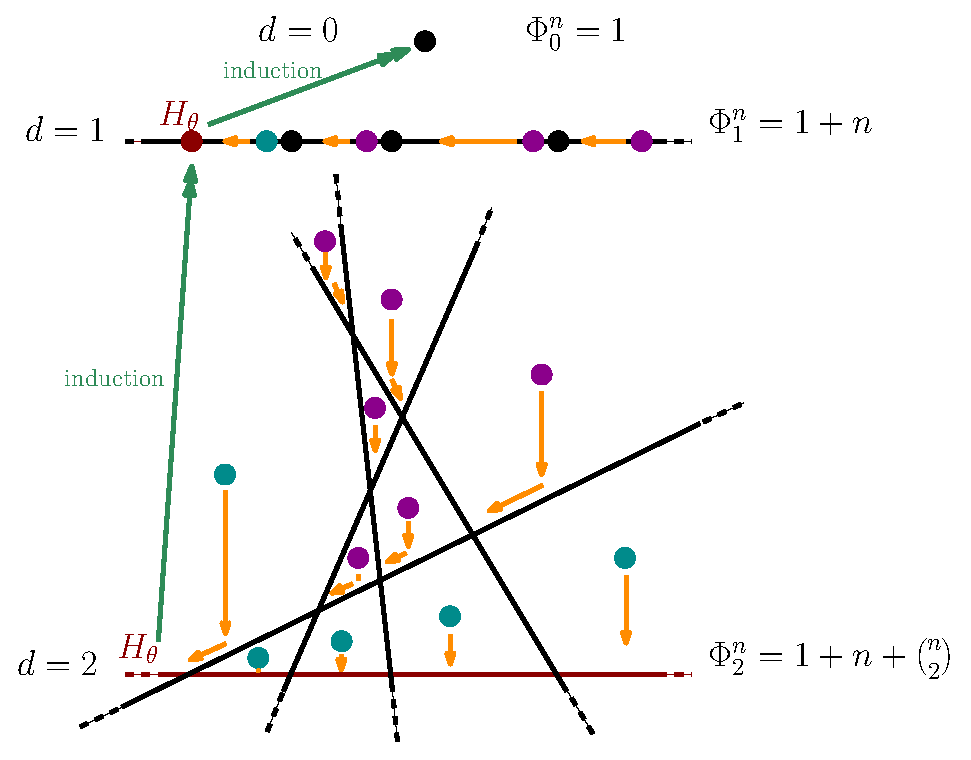
\includegraphics[width=0.7\textwidth,trim=-50 0 0 0]{fig/x+y/buck/arrangement}
\caption{Induction steps in the second proof of \citet*{matousek:2002}.}
\label{fig:xy:buck:arrangement}
\end{figure}

\begin{proof}
We assume a partition of space \(\R^d\) by a simple arrangement of \(n\)
hyperplanes, \ie all \(d\) hyperplanes intersect in exactly one point and no
more than \(d\) hyperplanes are incident to a point.

\ref{fig:xy:buck:arrangement} shows that we can divide the set of cells in two
disjoint subsets, \(\L\) and \(\U\). The subset \(\L\) is constituted of cells that are
intersected by an imaginary additional hyperplane \(H_{\theta}\) having all
\(\binom{n}{d}\) intersections of the arrangement on one of its sides (either
\(H_{\theta}^{+}\) or \(H_{\theta}^{-}\)) and thus intersecting all the \(n\)
hyperplanes of the arrangement on one side of the vertices. The subset \(\U\) contains the
remaining cells.
\begin{displaymath}
\card{\L} = \Phi_{d-1}(n) \text{ since this is exactly the configuration for } \R^{d-1}
\end{displaymath}
\begin{displaymath}
\card{\U} = \binom{n}{d} \text{ since \dots}
\end{displaymath}
Imagine we drew a ball in each cell of the arrangement. If we pretend
\(H_{\theta}\) is the ground and we activate gravity, the balls in the cells of
\(\L\) would have fallen on \(H_{\theta}\). Each of them would be lying on a
\((d-1)\)-cell of the partition of \(H_{\theta}\) by the arrangement of the
intersections of each hyperplane of the arrangement with \(H_{\theta}\). The
balls in the cells of \(\U\) cannot fall on the ground since \(H_{\theta}\)
does not intersect the cells containing them. Balls in \(\U\) cells can thus
only end up in one of the \(\binom{n}{d}\) intersections of the \(n\)
hyperplanes.
\end{proof}

\citet*{matousek:2002} also shows that
\begin{displaymath}
\Phi_d(n) = \Phi_d(n-1) + \Phi_{d-1}(n-1)
\end{displaymath}
in the first, more rigorous, proof. The term \(\Phi_d(n-1)\) can be understood as the
number of cells of an arrangement of \(n-1\) hyperplanes that were existing
before the addition of an \(\nth{n}\) hyperplane. Then, the term \(\Phi_{d-1}(n-1)\)
counts the number of cells that are cut in two by the \(\nth{n}\) hyperplane.
